\subsection{Mikrocontroller}
\label{subsec:Mikrocontroller}

Der Mikrocontroller ist die Seele, das Gehirn der Maschine. Er muss in der Lage sein mit allen Komponenten auf der Platine zu kommunizieren, die Tasks zu verarbeiten und abhandeln. Der ATMega2560 übernimmt diese Aufgabe.

\paragraph{Schema}\mbox{}

Das Schema besteht aus dem Mikrocontroller IC8 mit den fünf Stützkondensatoren C62, bis C66 an den Spannungseingängen. Mit dem Full Swing Oscillator Crystal Y2 und den Kondensatoren C58 und C59 wird eine Frequenz von 16MHz generiert. Der Reset-Button 

\begin{figure}[!h]
\center
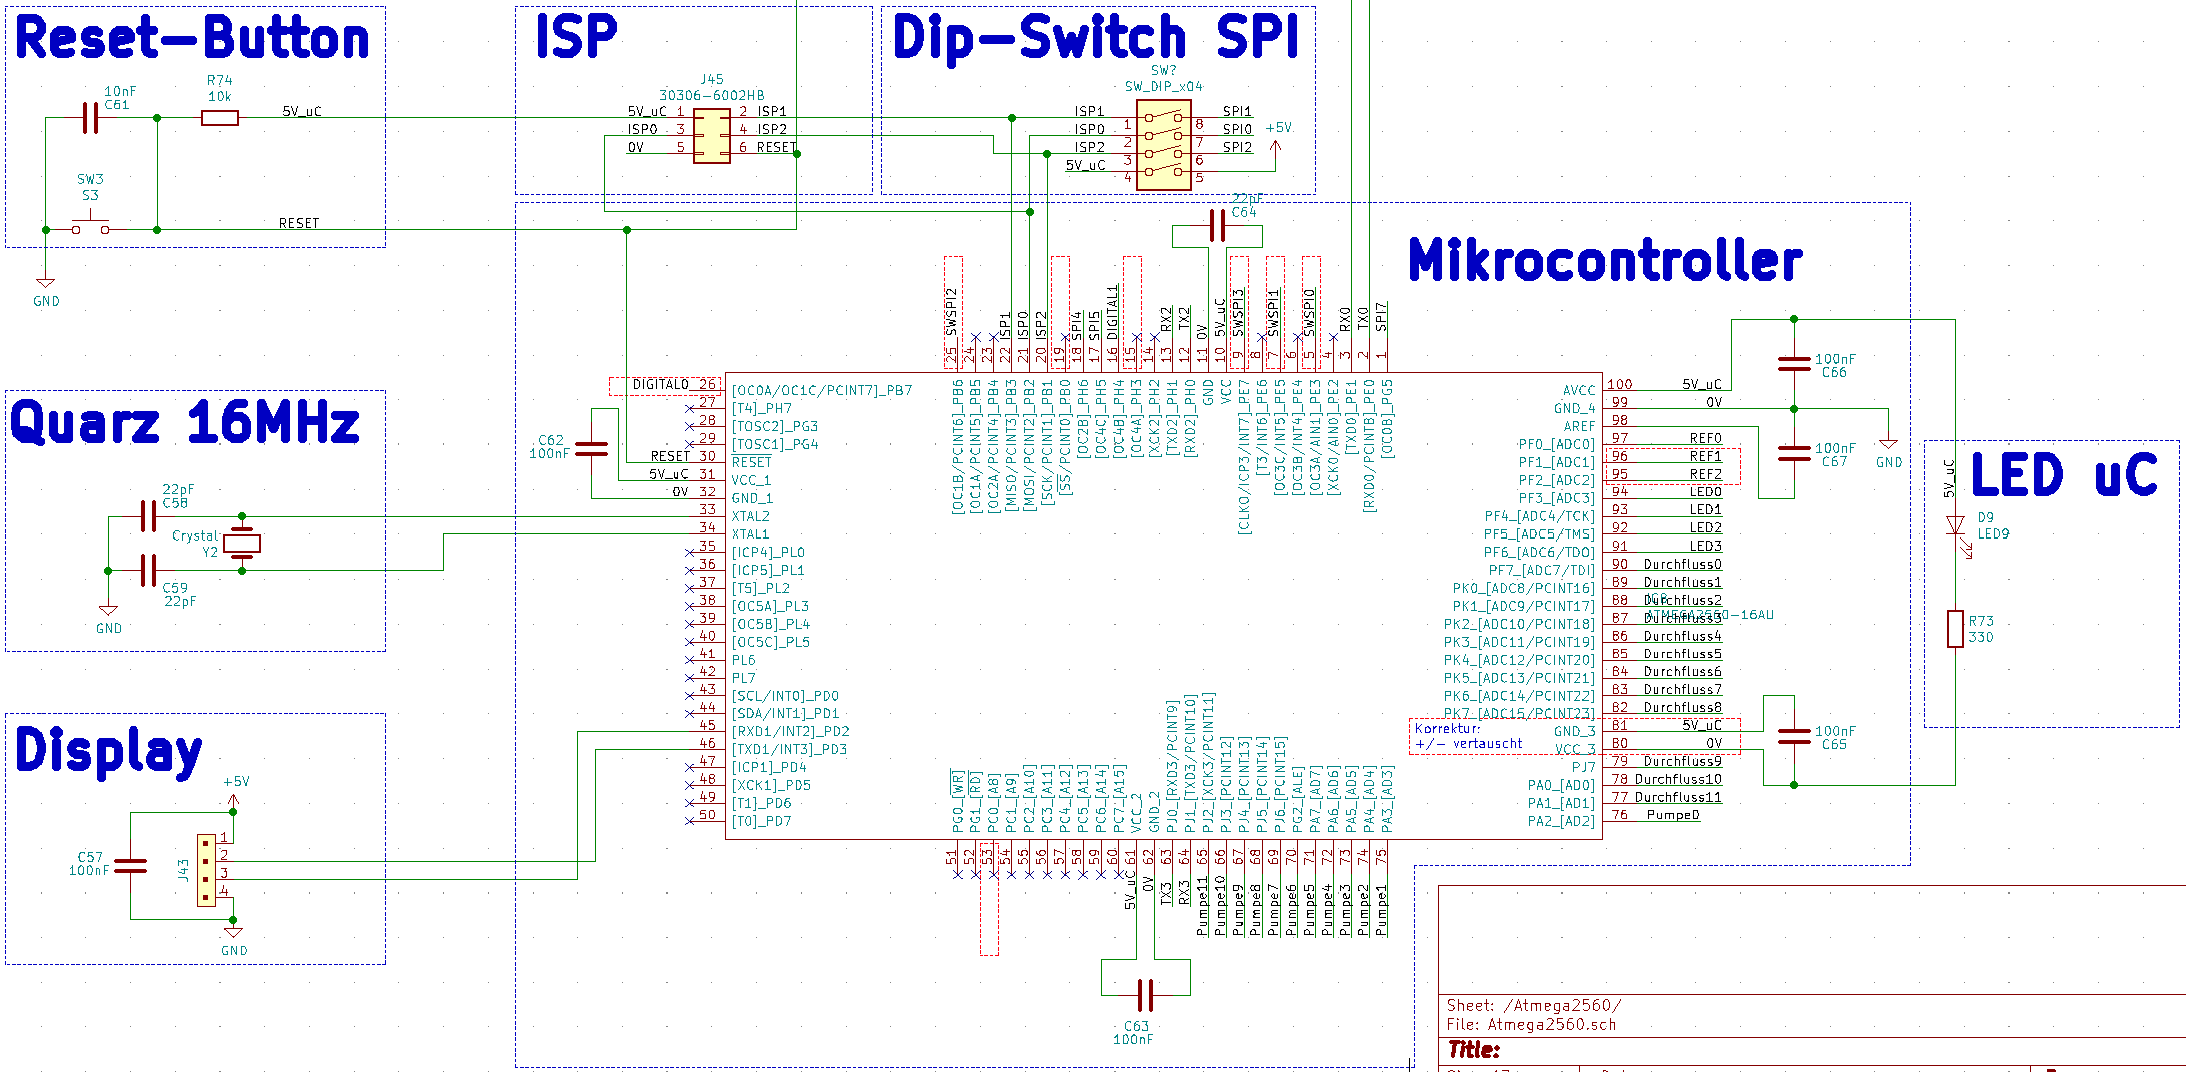
\includegraphics[width = \textwidth]{graphics/Schema_uC}
\caption{Schema Mikrocontroller}
\label{fig:Schema_uC}
\end{figure}

\paragraph{Funktionsbeschrieb der Schaltung}\mbox{}

